
%%%%%%%%%%%%%%%%%%%%%%%%%%%%%%%%%%%%%%%%%%%%%%%%%%%%%%%%%%%%%%%%%%%%%%%%
%    INSTITUTE OF PHYSICS PUBLISHING                                   %
%                                                                      %
%   `Preparing an article for publication in an Institute of Physics   %
%    Publishing journal using LaTeX'                                   %
%                                                                      %
%    LaTeX source code `ioplau2e.tex' used to generate `author         %
%    guidelines', the documentation explaining and demonstrating use   %
%    of the Institute of Physics Publishing LaTeX preprint files       %
%    `iopart.cls, iopart12.clo and iopart10.clo'.                      %
%                                                                      %
%    `ioplau2e.tex' itself uses LaTeX with `iopart.cls'                %
%                                                                      %
%%%%%%%%%%%%%%%%%%%%%%%%%%%%%%%%%%
%
%
% First we have a character check
%
% ! exclamation mark    " double quote  
% # hash                ` opening quote (grave)
% & ampersand           ' closing quote (acute)
% $ dollar              % percent       
% ( open parenthesis    ) close paren.  
% - hyphen              = equals sign
% | vertical bar        ~ tilde         
% @ at sign             _ underscore
% { open curly brace    } close curly   
% [ open square         ] close square bracket
% + plus sign           ; semi-colon    
% * asterisk            : colon
% < open angle bracket  > close angle   
% , comma               . full stop
% ? question mark       / forward slash 
% \ backslash           ^ circumflex
%
% ABCDEFGHIJKLMNOPQRSTUVWXYZ 
% abcdefghijklmnopqrstuvwxyz 
% 1234567890
%
%%%%%%%%%%%%%%%%%%%%%%%%%%%%%%%%%%%%%%%%%%%%%%%%%%%%%%%%%%%%%%%%%%%
%
%%novalidate

\documentclass[12pt,a4paper,final]{iopart}
\newcommand{\gguide}{{\it Preparing graphics for IOP journals}}
%Uncomment next line if AMS fonts required
\usepackage{iopams}
\usepackage{graphicx}
\usepackage[breaklinks=true,colorlinks=true,linkcolor=blue,urlcolor=blue,citecolor=blue]{hyperref}

% Custom for this paper
\bibliographystyle{iopart-num}
%\usepackage{amsmath,amssymb,amsfonts}
%\usepackage{mathtools}
% for \code color
\usepackage[dvipsnames]{xcolor}
\usepackage{todonotes}
\usepackage{menukeys}
\usepackage{siunitx}
\usepackage{listings}
% Pretty formating of c++ (see \cpp command)
\usepackage{xspace}
\newcommand*{\cpp}{C\ensuremath{++}\xspace}

\lstdefinelanguage{LAMMPS}{
    morekeywords={units,atom_style,lattice,region,create_box,create_atoms,pair_style,pair_coeff,neigh_modify,mass,velocity,fix,run, group every, equal, count, porosity, EDGE},
    sensitive=false, % keywords are not case-sensitive
    morecomment=[l]{//}, % l is for line comment
    morecomment=[s]{/*}{*/}, % s is for start and end delimiter
    morestring=[b]" % defines that strings are enclosed in double quotes
}

\lstset{
basicstyle=\small,
frame = single,
language=LAMMPS,
framexleftmargin=15pt,
xleftmargin=0.65cm,
xrightmargin=0.1cm}

% Highlighte inline code
\definecolor{light-gray}{gray}{0.95}
\definecolor{atomify-red}{rgb}{0.90196078 , 0.09803922, 0.29411765}
\definecolor{atomify-green}{rgb}{0.23529412 , 0.70588235, 0.29411765}
\definecolor{atomify-yellow}{rgb}{0.8,  0.70588235,  0.07843138}
\definecolor{atomify-blue}{rgb}{0.00000000 , 0.50980392, 0.78431373}
%\newcommand{\code}[1]{\mbox {\texttt{#1}}}
\newcommand{\code}[1]{\colorbox{light-gray}{\color{RawSienna}\texttt{#1}}}

\begin{document}

\title{Increased productivity using Atomify - a real-time LAMMPS visualizer}

\author[cor1]{Anders Hafreager$^{1}$}
\eads{\mailto{anderhaf@fys.uio.no}, \mailto{andershaf@gmail.com}}

\author{Svenn-Arne Dragly$^{1}$}
\ead{s.a.dragly@fys.uio.no}
\address{$^1$Department of Physics - University of Oslo\\Sem S{\ae}lands vei 24, NO-0316, Oslo, Norway}

\begin{abstract}
The typical workflow when running atomistic simulations includes working with several programs.
A text editor is needed to create and modify the scripts, the terminal to run the simulation, and programs like VMD or Ovito to visualize the system over time.
If physical quantities are computed, the data is often plotted using programming languages like MATLAB or Python,
where additional scripts must be used.
This is a tedious process, especially for teaching purposes and for people who are new in the field.
We here introduce Atomify; a high performance real-time visualizer for atomistic simulations that can simulate and render more than one million atoms with excellent frame rate on modern hardware.
Atomify supports OpenMP acceleration, GPU acceleration, real-time plotting of physical quantities, and an easy-to-use code editor in one single application.
It currently uses LAMMPS as physics engine, but it can be extended to support other codes like GROMACS, NAMD or CHARMM.
Atomify is open-source software (GPL) written in C++ using the Qt framework and can be downloaded from \url{https://github.com/ovilab/atomify}.
\end{abstract}

%Uncomment for PACS numbers title message
\pacs{00.00, 20.00, 42.10}
% Keywords required only for MST, PB, PMB, PM, JOA, JOB? 
\vspace{2pc}
% Comment out if separate title page not required
%\maketitle

\section{Introduction}

Over the past decades, users of LAMMPS\cite{Plimpton1995Fast} and other molecular dynamics simulators such
as GROMACS\cite{berendsen1995gromacs}, NAMD\cite{nelson1996namd} and CHARMM\cite{brooks2009charmm} have
typically written scripts in a text editor and run the scripts by passing them to the simulator on the command line.
The simulator in turn writes the results to disk and the user analyzes the results
by reading the files manually or passing them to other programs.

With the arrival of software like Rasmol\cite{sayle1995rasmol} and VMD\cite{Humphrey1996Vmd},
it became easy to both visualize the trajectories and analyze physical quantities such as the radial distribution function.
VMD came with support both for reading trajectories from file and attaching to a
running process using MDComm\cite{nelson1995mdscope} and a supported simulator such as NAMD\cite{nelson1996namd}.
Although this enabled real-time visualization, the workflow still involved using all these different programs which is still a problem today.

Analysis of simulations is often done as a postprocessing step where the trajectories and other per-atom quantities (velocity, stress etc.)
are loaded into an analysis tool written by researchers themselves. About 10 years ago, a new visualization tool called OVITO was released \cite{Stukowski2009Visualization},
with a powerful modifier pipeline where input data can be processed and manipulated as a series of building blocks.
These building blocks can be used to calculate new properties and atoms can be colored thereafter.

Scalar quantities such as temperature, pressure and number of atoms in a specific state are often printed to a
text file. Researchers often write their own plotting scripts in languages like MATLAB or Python
to see how these quantities evolve with time.

In combination, the text editors, the simulators, the visualization software, and the programming
languages like MATLAB and Python define the workflow of a typical researcher in computational
materials science.
While this is a powerful workflow in well-established simulations,
it is tedious for prototyping new ideas.
This workflow requires a fairly large amount of context switching,
moving from the text editor to the terminal to run the simulation,
waiting for the results, and then finally being able to study them using the analysis
and visualization tools.

Here, we present Atomify, a software that integrates script editing,
visualization and analysis into one tool.
Atomify has detailed knowledge about the inner workings of LAMMPS,
which makes it capable not only of visualizing the simulation results,
but also how the simulation is defined in terms of different groups and regions.

It is especially useful during development of new scripts, but can be used
to run full, publication-ready simulations with minimal simulation overhead.
The current implementation only supports LAMMPS as a simulator, but is written in a general
way so integrating other codes is a simple task.

\begin{figure}
	\centering
	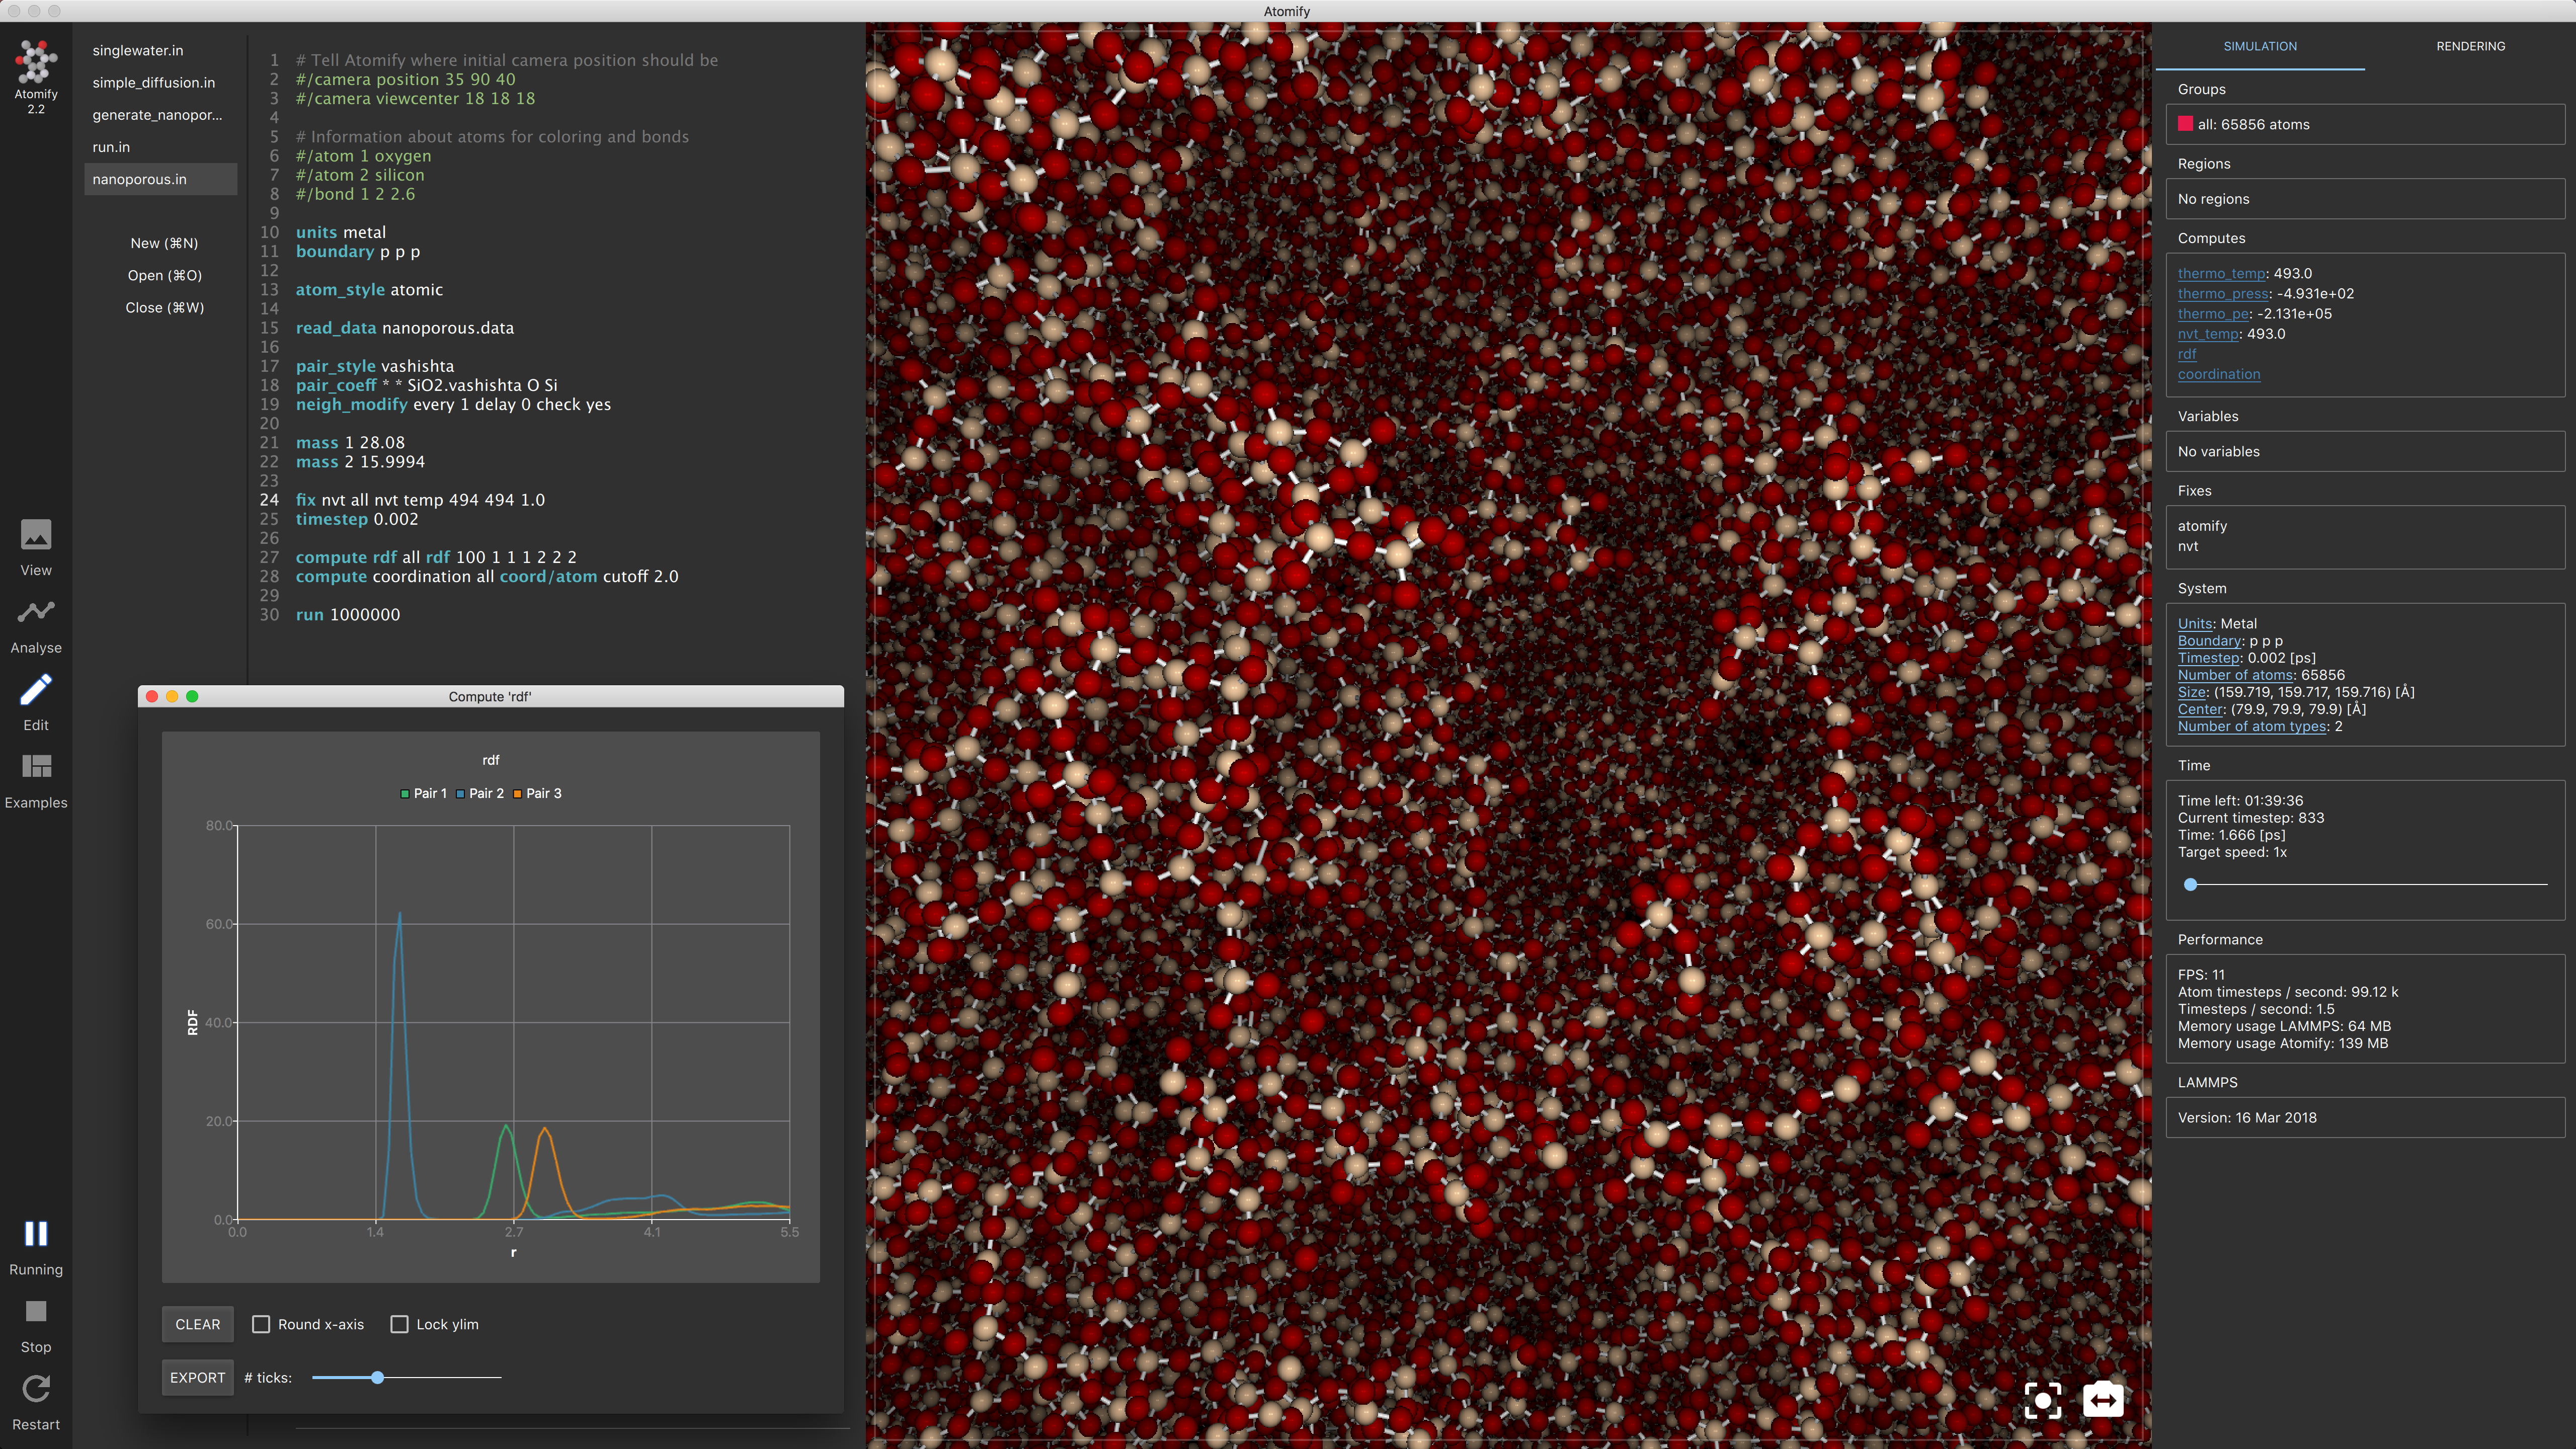
\includegraphics[width=\textwidth]{gui.png}
	\caption{%
    Overview of the Graphical User Interface (GUI) in Atomify.
    The toolbar (1) is used to change between the different modes, such as
    editing, viewing and analyzing the running simulation,
    in addition to playback controls.
    The file browser (2) contain the list of open LAMMPS scripts or data files.
    The text editor (3) provides code highlighting.
    The viewport (4) shows the current simulation.
    The simulation properties (5) shows the simulations details, gives access to
    LAMMPS objects such as groups, regions and computes, and the rendering
    properties (6) lets you change the viewport settings, such as lighting and
    draw mode.
    TODO: Add numbers to figure.
    }
	\label{fig:gui}
\end{figure}

In this paper we will go through a case study, an example simulation, where we
use many of the useful features Atomify provides.
We start by discussing the GUI in section \ref{sec:features} where the main features are summarized.
In section \ref{sec:casestudy}, the case study is introduced where we go through a typical example
of a simulation that uses regions and groups to perform different integration on different atoms.
Common pitfalls which are easily picked up with Atomify are shown.

\begin{figure}[htp!]
	\centering
	\includegraphics[width=0.5\textwidth]{figures/rightbar.pdf}
	\caption{
		The \textit{Simulation summary} is a powerful feature in Atomify where relevant
		properties from LAMMPS is presented real-time.
		In a), a list of all groups defined is shown with the current atom count.
		b) shows all defined regions. Each group and region can be hovered so that atoms
		are colored after what group / region they are in. If an atom is in multiple
		groups or regions, they will get the color of the latest one defined.
		The color boxes can be clicked which will either always highlight the atoms in a certain group or region,
		or if clicked again, hide all of them.
		In c) and d), a list of all variables and computes is shown. If a variable or compute
		produces a scalar, the current value is shown as can be seen with all the variables.
		By clicking the name, a plot will show up showing the time evolution of that quantity.
		If a per-atom variable or compute is hovered, all atoms will be colored according to their
		current scalar value and a histogram over these values is shown if clicked.
		The result of hovering atoms defined by the groups in our case study is shown in figure \ref{fig:cylinder_simulation}.
    }
	\label{fig:rightbar}
\end{figure}

\section{\label{sec:features}Summary of features}
Atomify was designed to improve the workflow as its main goal.
Focusing on minimizing the number of context switches and mouse clicks reduces
the overhead between creativity and immediate results from a simulation.
It has a script editor, visualization window and a summary panel so all relevant parts
of a simulation can be on the screen at the same time.

Any changes to the script like defining regions or groups,
testing temperatures, size of simulation box or inserting atoms can
quickly be verified since the visualization shows the real-time state of the simulator.
Rerunning the current script can be done by pressing \keys{Ctrl+R} (\keys{cmd+R} on macOS).

How the pressure, radial distribution function or some other
complicated variable evolves over time is easily understood
since these can be plotted real-time with a simple click in the list of variables.
Bonds between atoms in a molecule is automatically extracted from LAMMPS, or can
be defined as a distance threshold between atom types.
Regions and groups can be highlighted or hidden which is useful to focus on some parts of a system.
Rendering periodic copies can be done to study features near a periodic boundary condition.

Per-atom scalar quantities can be used to color each atom based its value.
For instance, \code{compute cna/atom}\cite{faken1994systematic, tsuzuki2007structural} can be used to identify the crystal structure an atom is a part of.
It gives each atom an integer value in the range [1,5] representing FCC, HCP, BCC, Icosohedral or unknown crystal structure.
\code{compute displace/atom} can be used to see how far each atom has moved and \code{compute stress/atom} gives the local stress in the system.
These values can be used as input to \code{fix ave/atom} to get time averaged values to reduce noise.
Coloring each atom based on these values can give great insight when it is available with a single mouse click.

Although LAMMPS is mostly used to study molecular dynamics, it can also be used to
study monte carlo simulations\cite{frenkel2001understanding} and granular
materials\cite{brilliantov1996model, silbert2001granular, zhang2005jamming},
both of which work very well in Atomify since they are particle based simulations.

Atomify supports rendering of spheres and cylinders representing atoms and bonds.
It is done using the powerful Qt3D engine with custom visualization techniques such as
billboard raytracing\cite{tarini2006ambient} and screen space ambient occlusion\cite{bavoil2008screen}
for improved dynamic depth perception. This allows a large amount of atoms and molecules being rendered with excellent framerate.
The liming factor is the simulation itself since force calculation is a heavy task.

The Atomify GUI is shown in figure \ref{fig:gui} where \todo{short summary of GUI}.
This turns out to improve the workflow substantially.
In addition, Atomify comes with multiple examples,
many of which have been made by members of the LAMMPS community.

\section{\label{sec:casestudy}Case study: flow through a narrow nanotube}
\todo[inline]{More references in here?}
The features of Atomify is best demonstrated through a case study where many of
them are useful to obtain a productive workflow during script development.
We have chosen to create a system with fluid flow inside a tight nanochannel.
This involves creating a somewhat complicated initial geometry with multiple regions
where we apply different rules such as a dissipative thermostat, constant force mimicking
applied pressure gradient, and frozen atoms to avoid net momentum of the solid.
We will create two different atom types so we can have a gas phase and a solid phase at the same temperature.

Fluid flow in porous media is often characterized with its permeability - the inverse flow resistance of a material.
The permeability can be measured using Darcy's law when applying a pressure gradient $\nabla P$.
In Darcy's law, the permeability is assumed to only depend on the material and its geometry.
However, this turns out not being the case for dilute
gases where the measured permeability changes as a function of pressure\cite{klinkenberg1941permeability}.
This is called the Klinkenberg effect.

The discrepancy is explained by the fact that at low pressures, the fluid velocity
at the boundary is non-zero, i.e. we have a non-slip boundary condition.
A non-slip boundary condition is a good approximation for liquids in larger pores,
but if the channel size $R$ is of the same order,
or larger, as the mean free path $\lambda$ of the fluid, it is no longer true.

The ratio between the mean free path and the channel size is quantified through
the Knudsen number, $\text{Kn} = \lambda / R$, and can be used to apply the Klinkenberg correction\cite{klinkenberg1941permeability}
to correctly describe the \textit{effective permeability} as a function of pressure in the high Knudsen number limit.

\begin{figure}
	\centering
	\includegraphics[width=0.75\textwidth]{lj_flow/configuration.png}
	\caption{
		Initial configuration in our case study simulation.
		A periodic box consisting of $(40\times25\times25)$ FCC unit cells with reduced density $\rho^* = 0.8442$ where we will have gas flow in a cylinder with radius 10 (reduced length).
		The different colors indicate the regions of which different integration rules apply.
		Cyan atoms are fixed and do not move at all,
		whereas the purple atoms are thermalized with a Langevin\cite{schneider1978molecular} dissipative thermostat to mimick the heat exchange with the frozen bulk atoms.
		The orange and the yellow atoms are integrated normally, but the yellow gas atoms also have an applied constant acceleration representing the pressure gradient.
		Setting up and verifying the system is simple using Atomify due to i.e. the real-time coloring of groups and regions.
    }
	\label{fig:cylinder_simulation}
\end{figure}

In this case study, we will use Atomify to measure the velocity profile of a
gas inside a nanotube with varying density to observe
the slip velocity effect at low densities.
We will use the Lennard Jones potential with two different atom types.

We create the nanotube inside a solid with  $(60\times30\times30)$ FCC unit cells and reduced density $\rho^* = 0.975$.
This density was chosen so that the two atom types with the Lennard Jones coefficients specified below will coexist in different phases.
The fluid in the nanotube, or cylinder, will flow due to an induced pressure gradient, see figure \ref{fig:cylinder_simulation}.
Here we apply a pressure gradient $\nabla P$ in the $x$-direction on the gas atoms using a constant acceleration $a$ calculated as
\[
    a = \frac{\nabla P}{\rho_m},
\]
where $\rho_m$ is the mass density of the gas atoms and $\nabla P$ is the desired pressure gradient.
This represents a pressure difference $\Delta P$ over a small volume element $\Delta x$ on a cross-sectional area $\Delta y\Delta z$.

Applying an acceleration means adding energy to the system which in turn will increase the temperature and eventually melt the system.
To avoid this, we couple the solid to an external heat bath so the added energy can be transferred out from the system through a dissipative thermostat.

Even though we only apply a pressure gradient on the gas atoms, the induced momentum will be transferred
to the solid atoms which eventually will start moving in the positive $x$-direction, which is not desired.
The solid should be at rest since it is only the relative velocity between the gas and the solid that defines
the flow. We therefore freeze the outmost atoms (colored cyan in Fig \ref{fig:cylinder_simulation}).
To obtain this system, we divide the atoms into multiple cylindrical regions, which are integrated differently:

\begin{itemize}
	\item $r \leq 12$: applied pressure gradient
	\item $r \leq 23$: regular time integration
	\item $18 < r \leq 23$: dissipative Langevin thermostat
	\item $23 < r$: frozen.
\end{itemize}
The different radii are specified in reduced Lennard Jones units.

\subsection{Creating the initial geometry}
We create a new script in Atomify using \keys{\cmd+N}, and save it (\keys{\cmd+S}) as \code{run.in}.
Copy the following input script

\todo[inline]{Should we remove line numbers?}
\lstinputlisting[language=LAMMPS]{simple.in}
we will modify it part by part.
Here, we have a Lennard Jones solid with reduced density
$\rho^* = 0.975$, reduced masses $m_1^* = 4.0$, $m_2^* = 0.5$ with $(60\times30\times30)$
FCC unit cells and a cutoff of $2.5$. 
The force field parameters are chosen so that atoms of type 1
are in the solid phase with type 2 atoms being gas at reduced temperature $T^*=0.5$.
The two atom types are weakly coupled (small $\epsilon_{ij}$)so the gas atoms don't
stick too much to the surface which would prevent flow.

To make sure LAMMPS executes our modifiction before visualization is started,
we need to make sure that following additional commands happen \textit{before} the \code{run 1000} command.
If not, LAMMPS will run 1000 timesteps before getting to our changes.

To define the inner cylinder, we first specify the radius and the center before using the region command
\begin{lstlisting}
variable R equal 12
variable c equal $(ly*0.5)
region cylinder1 cylinder x $c $c $R EDGE EDGE
set region cylinder1 type 2
\end{lstlisting}
The region command will create a cylinder $C_1$ in the $x$-direction, with $(y,z)$-coordinates at the system center \code{\$c} with radius \code{\$R} using the full length of the system in the $x$-direction specified when using \code{EDGE}.
Atoms inside the region will also be changed to type 2 since these will be the gas atoms.

We now press \keys{\cmd+R} to run the simulation to see how it looks.
As shown in figure \ref{fig:rightbar}, we can hover the specified region to highlight the atoms in it.

\begin{figure}
	\centering
	\includegraphics[width=0.8\textwidth]{figures/initial_configuration.pdf}
	\caption{
		Several snapshots of the process of creating the simulation in our case study.
		This shows how one typically generate a geometry step by step where the immediate
		feedback is very useful to quickly discover mistakes.
		The wrongly placed cylinder is shown in a) whereas it is placed correctly in b).
		c) shows how the system looks after deleting atoms to obtain $\rho = 0.01$. The next cylinder $C_2$ is shown in d),
		and all regions (placed in groups) are shown in e). Here we have uniquely defined the purple shell which should have a dissipative thermostat.
		In f), the list of all groups defined in this system is shown with colors matching those of e). All figures are rendered with Atomify.
    }
	\label{fig:initial_configuration}
\end{figure}

When we hover the region, we immediately see that the cylinder is in fact not placed at the center of the system, as shown in figure \ref{fig:initial_configuration}a.
The reason is that LAMMPS operate with two different units, either the length unit or the lattice length unit. This is explained in the documentation, but is a common mistake.
Discovering mistakes like this is very easy using Atomify.

The problem here is that LAMMPS expects the values to be in \textit{lattice} units, i.e. multiples of the lattice constant.
Since we used \code{\$(0.5*lx)}, which gives the system length in actual lenght units, we need to specify \code{units box} in the region command.
We then rerun the simulation with \keys{\cmd+R} which gives the expected result in figure \ref{fig:initial_configuration}b.

Now that the region looks like we expect, we want to delete atoms to control the density.
The volume of the inner cylinder is $\pi R^2 L$ which can be calculated in LAMMPS with \code{variable V equal PI*v\_R*v\_R*lx}.
The command \code{delete\_atoms} can be used: \code{delete\_atoms porosity region-ID fraction seed},
where we need to specify the fraction of the existing atoms in that region we want to delete, and a random seed which can be any positive number.
Since we want to specify a certain density, we need to figure out how many atoms we
should delete which depends on the current number of atoms inside the region.

To count the number of atoms inside a region, we first create a group containing all the atoms in it, and then create a variable that counts them.
Assuming density $\rho_m = 0.1$, we can calculate the expected number inside the cylinder as $N = V\rho_m/m$,
where $V$ is the volume of the cylinder and $m$ is the mass of type 2 atoms.
The atoms inside the region can now be deleted with the following commands
\begin{lstlisting}
group cylinder1 region cylinder1
variable N_cyl equal count(cylinder1)
variable V equal PI*v_R*v_R*lx
variable rho_m equal 0.1
variable N_wanted equal $V*${rho_m}/0.5
variable delete_fraction equal (${N_cyl}-${N_wanted})/${N_cyl}
delete_atoms porosity cylinder1 ${delete_fraction} 1234
\end{lstlisting}
where we see the result by rerunning with \keys{\cmd+R} in figure \ref{fig:initial_configuration}c.

This is a powerful workflow with Atomify where changes quickly can be tested with immediate feedback.
Each time we add or change a command, we just rerun with \keys{\cmd+R} to see how it looks like.

The next step now is to create a larger cylinder $C_2$, the one containing the orange atoms in
figure \ref{fig:cylinder_simulation}, where regular time integration will take place.
This cylinder should have a slightly bigger radius and can be created with another region command:
\begin{lstlisting}
region cylinder2 cylinder x $c $c $(v_R+6) EDGE EDGE units box
\end{lstlisting}
Again press \keys{\cmd+R} to see the expected result in figure \ref{fig:initial_configuration}d.

Now we have the inner cylinder with the gas atoms defined as a region and the next cylinder shell (including the gas atoms) defined as another region.
We now want to create another shell, the one with the dissipative thermostat.
All the atoms with the dissipative thermostat, the inner shell and the gas will be integrated with the \code{fix nve} integrator.
We therefore create a larger cylinder $C_3$ with $r=23$ which will be the one defining the group for \code{fix nve}.
With all three regions defined, we also create groups which will be used in fixes
\begin{lstlisting}
region cylinder3 cylinder x $c $c $(v_R+11) EDGE EDGE units box
group cylinder1 region cylinder1
group cylinder2 region cylinder2
group cylinder3 region cylinder3
group nve region cylinder3
\end{lstlisting}
where we also have created the group \code{nve} for clarity.

We will use \code{fix langevin}\cite{schneider1978molecular} as the dissipative thermostat,
but it should only be applied on the outer shell defined by atoms being in $C_3$, but not in $C_2$.
Groups define sets on which we can apply regular set operations like union, intersection and subtraction.
We can obtain the outer shell with the command

\begin{lstlisting}
group langevin subtract cylinder3 cylinder2
group frozen subtract all cylinder3
group gas dynamic all region cylinder1 every 1
\end{lstlisting}

We here also created the group \code{frozen}, which contains only the outmost atoms,
and the group \code{gas} which is dynamic since atoms may go in and out, and we want
to only apply a force on the ones in the inner cylinder $C_1$ at any point in time.
The frozen atoms will not move at all and make sure that the system does not start 
moving due to momentum transfer from the gas particles.

These groups are highlighted in figure \ref{fig:initial_configuration}e by hovering the
box containing all the groups in Atomify as shown in figure \ref{fig:initial_configuration}f.
The colors of the atoms match the group list in figure \ref{fig:initial_configuration}f,
where the order of coloring is the same as they were defined in the script.
Although one group is colored green, we don't see any green atoms (\code{cylinder1})
since all of them also are in the groups \code{cylinder2}, \code{cylinder3}, \code{nve} and \code{gas},
which overrides the color.

\subsection{Physical setup}
Now that we have managed to set up the system geometrically, 
we need to apply different actions, or fixes, on them.
First, we apply the time integration \code{fix nve} which
should happen on all atoms within $C_3$ (remember that we created the group \code{nve} for this)
, then the thermostat \code{fix langevin}

\begin{lstlisting}
fix nve nve nve
fix langevin langevin langevin 1.0 1.0 1.0 12345
compute displacement all displace/atom
\end{lstlisting}

The syntax for fixes is \code{fix ID groupID style args}, so the above fixes have the same name as both the groups and the fix style.
\code{fix langevin} takes at least 4 arguments \textit{Tstart, Tstop, Tdamp, seed}, i.e.
the temperature in the beginning of a simulation, the temperature at the end (timesteps in between get a linearly
interpolated temperature between these values), a damping parameter which controls how strongly the thermal bath interacts with the system.
It also needs a random seed due to the random nature of the Langevin thermostat as discussed in \cite{schneider1978molecular}.
Finally, we have added another compute that measures the displacement per atom.
In Atomify, we can hover this compute in the list of computes which will color each atom according to their displacement since $t=0$.
This works for any \textit{per-atom} compute or variable.

\begin{figure}
	\centering
	\includegraphics[width=0.8\textwidth]{lj_flow/07_moving.png}
	\caption{
		We see the expected moving atoms inside the $C_3$ cylinder.
		The atoms are colored based on their displacement (measured in reduced length units).
		We confirm that the outmost atoms are frozen, which we read from dark blue color mapping to 0 displacement.
		The moving atoms in the solid are blue, but brighter than the frozen ones which is expected due to their thermal vibrations.
		Inside the inner cylinder we see that the gas moves more freely since these atoms are not bounded.
    }
	\label{fig:moving_atoms}
\end{figure}

By rerunning again (\keys{\cmd+R}), we can confirm that the system behaves as expected.
In figure \ref{fig:moving_atoms}, we see that the outmost atoms are completely frozen (dark blue represents zero displacement),
the ones in the solid are also blue, but brighter, since they have moved a little bit through thermal vibrations in the lattice.
The inner cylinder contains gas atoms which move more freely, as seen from the colors being in the upper part of the color map.

The only remaining part now is to set up the commands that will apply the pressure gradient and measure the radial velocity profile.

\subsection{Measurement setup}
We will use the built-in binning feature in LAMMPS called \textit{chunks}, a very general concept where you assign a \code{chunkID} to each atom
based on its position. LAMMPS supports multiple different \textit{chunk styles}, one of which is cylinder.
In the cylinder binning, we choose the same properties as for a cylinder region (center, length etc.), but also the binsize in the length direction and how many radial bins we want.
We only want one bin in the flow direction since we only want to measure the radial velocity profile.
The command for giving each atom a \code{chunkID} is\footnote{The \& is used to continue the command on the next line since it is quite long.}
\begin{lstlisting}
compute chunk all chunk/atom bin/cylinder x lower &
$(lx) $c $c 0 $R 30 units box
\end{lstlisting}
It will create 30 radial bins for $r\in (0, R)$, where $R$ is the radius of the inner cylinder.
The final command we will use is the \code{fix ave/chunk} where we can get a smooth averaged velocity profile sampled over many timesteps.
To obtain this, we use
\begin{lstlisting}
fix vx all ave/chunk 10 10 100 chunk vx ave running
\end{lstlisting}
Here we use every 10th value to sample the velocity profile, keeping all samples to sum them into a larger histogram.
This fix will appear in the list of fixes in the \textit{Simulation summary} just as groups, regions, computes and variables.
When we click it, we will get the figure shown in figure \ref{fig:velocity_profile1}.

\begin{figure}
	\centering
	\includegraphics[width=0.8\textwidth]{lj_flow/08_velocity_profile1.png}
	\caption{
		The velocity profile for a Lennard Jones gas inside a nanochannel of radius 8.7 (reduced units).
		Since the wall also is made of Lennard Jones atoms, some of the wall atoms
		This figure is made using the Atomify real-time plotter which can show any scalar value defined in LAMMPS
		as compute, fix or variable.
    }
	\label{fig:velocity_profile1}
\end{figure}
\todo{Create fig 6 with both one single velocity profile and MATLAB plot of all of them. Maybe W/H = 0.5?}
\subsection{Results}
We conclude this case study with a series of simulations of the system described above for different densities $\rho$.
Each simulation runs 10000 timesteps before we export the plots from \code{fix vx} to MATLAB using the Export function seen in figure \ref{fig:velocity_profile1}.
All these plots are now merged into a final figure which is shown in figure \ref{fig:velocity_profiles}.
It is here evident that the velocity near the boundary is not zero, which is the reason why the permeability is much higher for dilute gases than dense liquids.
This is, as mentioned earlier, called the Klinkenberg effect\cite{klinkenberg1941permeability}.

\section{\label{sec:discussion}Discussion}
In this paper we have presented Atomify, an new software that reduces the amount of context switches and mouse clicks
when developing new simulation scripts.
As of today, only LAMMPS is supported as the physical simulator, but other codes can easily be integrated
due our general implementation with no assumpetion about the underlying code except atom positions.
The communication overhead is minimized since LAMMPS runs in the same process as Atomify, sharing the memory.

\section{Availability}
Atomify is available on Linux and MacOS and can be downloaded from
\href{https://ovilab.net/atomify}{http://ovilab.net/atomify}.
A lightweight version of Atomify is also available for mobile devices running
Android or iOS.

\todo[inline]{Potentially future work, emscripten, webassembly? emscripten has a proceedings paper.}

\section{Acknowledgments}
Statoil etc.

\section*{References}
\bibliography{Remote}

%
%\begin{thebibliography}{10}
%\bibitem{ref1} J.~Doe, Article name, \textit{Phys. Rev. Lett.}

%\bibitem{ref2} J.~Doe, J. Smith, Other article name, \textit{Phys. Rev. Lett.}

%\bibitem{web} \href{http://www.google.pl}{www.google.pl}
%\end{thebibliography}

\end{document}

